% Options for packages loaded elsewhere
\PassOptionsToPackage{unicode}{hyperref}
\PassOptionsToPackage{hyphens}{url}
%
\documentclass[
]{article}
\usepackage{ctex}
\usepackage{geometry}
\geometry{a4paper,left=2.8cm,right=2.8cm,top=3cm,bottom=2.5cm}
\usepackage{amsmath,amssymb}
\usepackage{graphicx}
\let\oldincludegraphics\includegraphics
\renewcommand{\includegraphics}[2][]{\begin{center}\oldincludegraphics[#1]{#2}\end{center}}
\usepackage{iftex}
\ifPDFTeX
  \usepackage[T1]{fontenc}
  \usepackage[utf8]{inputenc}
  \usepackage{textcomp} % provide euro and other symbols
\else % if luatex or xetex
  \usepackage{unicode-math} % this also loads fontspec
  \defaultfontfeatures{Scale=MatchLowercase}
  \defaultfontfeatures[\rmfamily]{Ligatures=TeX,Scale=1}
\fi
\usepackage{lmodern}
\ifPDFTeX\else
  % xetex/luatex font selection
\fi
% Use upquote if available, for straight quotes in verbatim environments
\IfFileExists{upquote.sty}{\usepackage{upquote}}{}
\IfFileExists{microtype.sty}{% use microtype if available
  \usepackage[]{microtype}
  \UseMicrotypeSet[protrusion]{basicmath} % disable protrusion for tt fonts
}{}
\makeatletter
\@ifundefined{KOMAClassName}{% if non-KOMA class
  \IfFileExists{parskip.sty}{%
    \usepackage{parskip}
  }{% else
    \setlength{\parindent}{0pt}
    \setlength{\parskip}{6pt plus 2pt minus 1pt}}
}{% if KOMA class
  \KOMAoptions{parskip=half}}
\makeatother
\usepackage{xcolor}
\usepackage{color}
\usepackage{fancyvrb}
\newcommand{\VerbBar}{|}
\newcommand{\VERB}{\Verb[commandchars=\\\{\}]}
\DefineVerbatimEnvironment{Highlighting}{Verbatim}{commandchars=\\\{\}}
% Add ',fontsize=\small' for more characters per line
\newenvironment{Shaded}{}{}
\newcommand{\AlertTok}[1]{\textcolor[rgb]{1.00,0.00,0.00}{\textbf{#1}}}
\newcommand{\AnnotationTok}[1]{\textcolor[rgb]{0.38,0.63,0.69}{\textbf{\textit{#1}}}}
\newcommand{\AttributeTok}[1]{\textcolor[rgb]{0.49,0.56,0.16}{#1}}
\newcommand{\BaseNTok}[1]{\textcolor[rgb]{0.25,0.63,0.44}{#1}}
\newcommand{\BuiltInTok}[1]{\textcolor[rgb]{0.00,0.50,0.00}{#1}}
\newcommand{\CharTok}[1]{\textcolor[rgb]{0.25,0.44,0.63}{#1}}
\newcommand{\CommentTok}[1]{\textcolor[rgb]{0.38,0.63,0.69}{\textit{#1}}}
\newcommand{\CommentVarTok}[1]{\textcolor[rgb]{0.38,0.63,0.69}{\textbf{\textit{#1}}}}
\newcommand{\ConstantTok}[1]{\textcolor[rgb]{0.53,0.00,0.00}{#1}}
\newcommand{\ControlFlowTok}[1]{\textcolor[rgb]{0.00,0.44,0.13}{\textbf{#1}}}
\newcommand{\DataTypeTok}[1]{\textcolor[rgb]{0.56,0.13,0.00}{#1}}
\newcommand{\DecValTok}[1]{\textcolor[rgb]{0.25,0.63,0.44}{#1}}
\newcommand{\DocumentationTok}[1]{\textcolor[rgb]{0.73,0.13,0.13}{\textit{#1}}}
\newcommand{\ErrorTok}[1]{\textcolor[rgb]{1.00,0.00,0.00}{\textbf{#1}}}
\newcommand{\ExtensionTok}[1]{#1}
\newcommand{\FloatTok}[1]{\textcolor[rgb]{0.25,0.63,0.44}{#1}}
\newcommand{\FunctionTok}[1]{\textcolor[rgb]{0.02,0.16,0.49}{#1}}
\newcommand{\ImportTok}[1]{\textcolor[rgb]{0.00,0.50,0.00}{\textbf{#1}}}
\newcommand{\InformationTok}[1]{\textcolor[rgb]{0.38,0.63,0.69}{\textbf{\textit{#1}}}}
\newcommand{\KeywordTok}[1]{\textcolor[rgb]{0.00,0.44,0.13}{\textbf{#1}}}
\newcommand{\NormalTok}[1]{#1}
\newcommand{\OperatorTok}[1]{\textcolor[rgb]{0.40,0.40,0.40}{#1}}
\newcommand{\OtherTok}[1]{\textcolor[rgb]{0.00,0.44,0.13}{#1}}
\newcommand{\PreprocessorTok}[1]{\textcolor[rgb]{0.74,0.48,0.00}{#1}}
\newcommand{\RegionMarkerTok}[1]{#1}
\newcommand{\SpecialCharTok}[1]{\textcolor[rgb]{0.25,0.44,0.63}{#1}}
\newcommand{\SpecialStringTok}[1]{\textcolor[rgb]{0.73,0.40,0.53}{#1}}
\newcommand{\StringTok}[1]{\textcolor[rgb]{0.25,0.44,0.63}{#1}}
\newcommand{\VariableTok}[1]{\textcolor[rgb]{0.10,0.09,0.49}{#1}}
\newcommand{\VerbatimStringTok}[1]{\textcolor[rgb]{0.25,0.44,0.63}{#1}}
\newcommand{\WarningTok}[1]{\textcolor[rgb]{0.38,0.63,0.69}{\textbf{\textit{#1}}}}
\usepackage{longtable,booktabs,array}
\usepackage{calc} % for calculating minipage widths
% Correct order of tables after \paragraph or \subparagraph
\usepackage{etoolbox}
\makeatletter
\patchcmd\longtable{\par}{\if@noskipsec\mbox{}\fi\par}{}{}
\makeatother
% Allow footnotes in longtable head/foot
\IfFileExists{footnotehyper.sty}{\usepackage{footnotehyper}}{\usepackage{footnote}}
\makesavenoteenv{longtable}
\usepackage{graphicx}
\makeatletter
\def\maxwidth{\ifdim\Gin@nat@width>\linewidth\linewidth\else\Gin@nat@width\fi}
\def\maxheight{\ifdim\Gin@nat@height>\textheight\textheight\else\Gin@nat@height\fi}
\makeatother
% Scale images if necessary, so that they will not overflow the page
% margins by default, and it is still possible to overwrite the defaults
% using explicit options in \includegraphics[width, height, ...]{}
\setkeys{Gin}{width=0.5\textwidth,keepaspectratio}
% Set default figure placement to htbp
\makeatletter
\def\fps@figure{htbp}
\makeatother
\setlength{\emergencystretch}{3em} % prevent overfull lines
\providecommand{\tightlist}{%
  \setlength{\itemsep}{0pt}\setlength{\parskip}{0pt}}
\setcounter{secnumdepth}{-\maxdimen} % remove section numbering
\ifLuaTeX
  \usepackage{selnolig}  % disable illegal ligatures
\fi
\IfFileExists{bookmark.sty}{\usepackage{bookmark}}{\usepackage{hyperref}}
\IfFileExists{xurl.sty}{\usepackage{xurl}}{} % add URL line breaks if available
\urlstyle{same}
\hypersetup{
  hidelinks,
  pdfcreator={LaTeX via pandoc}}

\author{}
\date{}

\begin{document}

\hypertarget{review-of-the-course-r-for-data-science-part-02talk-05-08}{%
\section{Review of the course ``R for Data Science'' Part 02(Talk
05\textasciitilde{}
08)}\label{review-of-the-course-r-for-data-science-part-02talk-05-08}}

\textbf{By Haoran Nie @ HUST Life ST}

This work is licensed under CC BY-NC-SA 4.0

\begin{center}\rule{0.5\linewidth}{0.5pt}\end{center}

To reduce the size, all the codes listed will \emph{\textbf{NOT}}
include the output as picture.

\hypertarget{r-for-bioinformatics-data-wrangler-part-1}{%
\section{R for bioinformatics, data wrangler, part
1}\label{r-for-bioinformatics-data-wrangler-part-1}}

\begin{quote}
Talk 05
\end{quote}

\hypertarget{toc}{%
\subsection{TOC}\label{toc}}

\hypertarget{pipe}{%
\subsubsection{pipe}\label{pipe}}

\hypertarget{dplyr}{%
\subsubsection{\texorpdfstring{\texttt{dplyr}}{dplyr}}\label{dplyr}}

\hypertarget{tidyr-part-1}{%
\subsubsection{\texorpdfstring{\texttt{tidyr}, part
1}{tidyr, part 1}}\label{tidyr-part-1}}

\hypertarget{pipe-in-r}{%
\subsection{Pipe in R}\label{pipe-in-r}}

\hypertarget{what-is-pipe-in-r}{%
\subsubsection{What is pipe in R?}\label{what-is-pipe-in-r}}

\begin{itemize}
\item
  Pipe is \texttt{\%\textgreater{}\%}.
\item
  It comes from the \texttt{magrittr} package by \textbf{Stefan Milton
  Bache}.
\item
  Packages in the \texttt{tidyverse} load
  \texttt{\%\textbackslash{}\textgreater{}\%} for you automatically, so
  you don\textquotesingle t usually load \texttt{magrittr} explicitly.
\item
  The essence is the passing of intermediate values.
\end{itemize}

\textbf{Example}

\begin{Shaded}
\begin{Highlighting}[]
\FunctionTok{library}\NormalTok{(tidyverse)}
\FunctionTok{library}\NormalTok{(magrittr)}
\NormalTok{a }\OtherTok{=}
 \FunctionTok{subset}\NormalTok{(swiss, Fertility }\SpecialCharTok{\textgreater{}} \DecValTok{20}\NormalTok{)}
\FunctionTok{cor.test}\NormalTok{(a}\SpecialCharTok{$}\NormalTok{Fertility, a}\SpecialCharTok{$}\NormalTok{Education)}
\end{Highlighting}
\end{Shaded}

The code above can be replaced by:

\begin{Shaded}
\begin{Highlighting}[]
\NormalTok{swiss }\SpecialCharTok{\%\textgreater{}\%}
  \FunctionTok{subset}\NormalTok{(., Fertility }\SpecialCharTok{\textgreater{}} \DecValTok{20}\NormalTok{) }\SpecialCharTok{\%\$\%}
  \FunctionTok{cor.test}\NormalTok{(Education, Fertility)}
\end{Highlighting}
\end{Shaded}

You should remember that almost \textbf{all} the funtions support pipe.

\hypertarget{other-kinds-of-pipe}{%
\subsubsection{Other kinds of pipe}\label{other-kinds-of-pipe}}

\begin{itemize}
\item
  \texttt{\%T\textgreater{}\%}: Return left-side values
\end{itemize}

\begin{itemize}
\item
  \texttt{\%\$\textgreater{}\%}: Attach \ldots{}
\end{itemize}

\begin{itemize}
\item
  \texttt{\%\textless{}\textgreater{}\%}
\end{itemize}

\hypertarget{attention}{%
\paragraph{\texorpdfstring{\textbf{ATTENTION}}{ATTENTION}}\label{attention}}

\begin{enumerate}
\def\labelenumi{\arabic{enumi}.}
\item
  The use of pipe makes the idea clearer;
\item
  Therefore, try to use \texttt{\%\textgreater{}\%} (which has a clear
  direction) instead of the other pipe, which has an unclear direction.
\end{enumerate}

\begin{center}\rule{0.5\linewidth}{0.5pt}\end{center}

\hypertarget{data-wrangler---dplyr}{%
\subsection{\texorpdfstring{Data Wrangler -
\texttt{dplyr}}{Data Wrangler - dplyr}}\label{data-wrangler---dplyr}}

\hypertarget{what-is-dplyr}{%
\subsubsection{\texorpdfstring{What is
\texttt{dplyr}?}{What is dplyr?}}\label{what-is-dplyr}}

\begin{itemize}
\item
  The next iteration of \texttt{plyr},
\item
  Focusing on only data frames (also tibble),
\item
  Row-based manipulation,
\item
  \texttt{dplyr} is faster and has a more consistent API.
\end{itemize}

\texttt{dplyr} provides a consistent set of verbs that help you
\textbf{solve the most common data manipulation challenges}:

\begin{itemize}
\item
  \href{https://dplyr.tidyverse.org/reference/select.html}{\texttt{select()}}
  Select columns, based on column name rules.
\item
  \href{https://dplyr.tidyverse.org/reference/filter.html}{\texttt{filter()}}
  Filter rows by rule.
\item
  \href{https://dplyr.tidyverse.org/reference/mutate.html}{\texttt{mutate()}}
  Add new column, calculated from other columns (no change in number of
  rows).
\item
  \href{https://dplyr.tidyverse.org/reference/summarise.html}{\texttt{summarise()}}
  Converts multiple values to a single value (via mean, median, sd,
  etc.), generating new columns (total number of rows is reduced,
  usually in conjunction with \texttt{group\_by}).
\item
  \href{https://dplyr.tidyverse.org/reference/arrange.html}{\texttt{arrange()}}
  Sorting the rows.
\end{itemize}

\begin{Shaded}
\begin{Highlighting}[]
\CommentTok{\# Read the file}
\FunctionTok{library}\NormalTok{(tidyverse)}
\NormalTok{mouse.tibble }\OtherTok{=}
  \FunctionTok{read\_delim}\NormalTok{(}
    \AttributeTok{file =} \StringTok{"data/mouse\_genes\_biomart\_sep2018.txt"}\NormalTok{,}
    \AttributeTok{delim =} \StringTok{"}\SpecialCharTok{\textbackslash{}t}\StringTok{"}\NormalTok{,}
    \AttributeTok{quote =} \StringTok{""}\NormalTok{,}
    \AttributeTok{show\_col\_types =} \ConstantTok{FALSE}
\NormalTok{  )}

\CommentTok{\# View mouse.tibble content}
\NormalTok{ttype.stats }\OtherTok{=}
\NormalTok{  mouse.tibble }\SpecialCharTok{\%\textgreater{}\%}
    \FunctionTok{count}\NormalTok{(}\StringTok{\textasciigrave{}}\AttributeTok{Transcript type}\StringTok{\textasciigrave{}}\NormalTok{) }\SpecialCharTok{\%\textgreater{}\%}
    \FunctionTok{arrange}\NormalTok{(}\SpecialCharTok{{-}}\NormalTok{n)}

\CommentTok{\# View mouse.tibble content, cont.}
\NormalTok{chr.stats }\OtherTok{=}
\NormalTok{  mouse.tibble }\SpecialCharTok{\%\textgreater{}\%}
    \FunctionTok{count}\NormalTok{(}\StringTok{\textasciigrave{}}\AttributeTok{Chromosome/scaffold name}\StringTok{\textasciigrave{}}\NormalTok{) }\SpecialCharTok{\%\textgreater{}\%}
    \FunctionTok{arrange}\NormalTok{(}\SpecialCharTok{{-}}\NormalTok{n)}
\end{Highlighting}
\end{Shaded}

\begin{center}\rule{0.5\linewidth}{0.5pt}\end{center}

\hypertarget{r-for-bioinformatics-data-wrangler-part-2}{%
\section{R for bioinformatics, data wrangler, part
2}\label{r-for-bioinformatics-data-wrangler-part-2}}

\begin{quote}
Talk 06
\end{quote}

\hypertarget{toc-2}{%
\subsection{TOC}\label{toc-2}}

\hypertarget{tidyr}{%
\subsubsection{\texorpdfstring{\texttt{tidyr}}{tidyr}}\label{tidyr}}

\begin{itemize}
\item
  \texttt{pivot\_longer()} to take the place of \texttt{gather}
\item
  \texttt{pivot\_wider()} to take the place of \texttt{spread}
\end{itemize}

\hypertarget{data-wrangler---tidyr}{%
\subsection{\texorpdfstring{Data Wrangler -
\texttt{tidyr}}{Data Wrangler - tidyr}}\label{data-wrangler---tidyr}}

You can get \texttt{tidyr} in the package set \texttt{tidyverse}, or
simply install it the first time you want to use it via
\texttt{install.packages("tidyr")}.

\hypertarget{the-usage-of-tidyr}{%
\subsubsection{\texorpdfstring{The usage of
\texttt{tidyr}}{The usage of tidyr}}\label{the-usage-of-tidyr}}

\begin{itemize}
\item
  Interconversion of wide and long data
\end{itemize}

\begin{Shaded}
\begin{Highlighting}[]
\NormalTok{\textasciigrave{}\textasciigrave{}\textasciigrave{}R}
\NormalTok{\# Eg 1}
\NormalTok{library(tidyverse)}
\NormalTok{grades2 =}
\NormalTok{	read\_tsv(file = "data/grades2.txt")}

\NormalTok{grades3 =}
\NormalTok{	grades2 \%\textgreater{}\% }
\NormalTok{	pivot\_longer( }
\NormalTok{    {-} name,}
\NormalTok{    names\_to = "course",}
\NormalTok{    values\_to = "grade"}
\NormalTok{  )}
\NormalTok{\textasciigrave{}\textasciigrave{}\textasciigrave{}}

\NormalTok{\textasciigrave{}\textasciigrave{}\textasciigrave{}R}
\NormalTok{\# Eg 2}
\NormalTok{grades3\_wide = grades3\_long \%\textgreater{}\% }
\NormalTok{  pivot\_wider(}
\NormalTok{    names\_from = "course",}
\NormalTok{    values\_from = "grade"}
\NormalTok{  )}
\NormalTok{\textasciigrave{}\textasciigrave{}\textasciigrave{}}
\end{Highlighting}
\end{Shaded}

\hypertarget{whats-the-difference-between-wide-and-long-data}{%
\subsubsection{What's the difference between wide and long
data?}\label{whats-the-difference-between-wide-and-long-data}}

Here are pros and cons of wide data:

\begin{itemize}
\item
  Pros:
\item
  Natural and easy to understand;
\item
  Cons:
\item
  Not easy to handle;

  \begin{itemize}
  \item
    More problematic when sparse.
  \end{itemize}
\end{itemize}

\hypertarget{if-you-meet-na-in-the-1st-example-you-can-do-like-this}{%
\subsubsection{\texorpdfstring{If you meet \texttt{NA} in the 1st
example, you can do like
this:}{If you meet NA in the 1st example, you can do like this:}}\label{if-you-meet-na-in-the-1st-example-you-can-do-like-this}}

\begin{Shaded}
\begin{Highlighting}[]
\NormalTok{grades3\_1 }\OtherTok{=}
\NormalTok{	grades3[}\SpecialCharTok{!}\FunctionTok{is.na}\NormalTok{(grades3}\SpecialCharTok{\$}\NormalTok{grade), ]}
\NormalTok{grades3\_2 }\OtherTok{=}
\NormalTok{	grades3[}\FunctionTok{complete.cases}\NormalTok{(grades3), ]}

\CommentTok{\# A better solution}
\NormalTok{grades3\_long }\OtherTok{=}\NormalTok{ grades2 }\SpecialCharTok{\%\textgreater{}\%} 
  \FunctionTok{pivot\_longer}\NormalTok{( }\SpecialCharTok{{-}}\NormalTok{ name, }
                \AttributeTok{names\_to =} \StringTok{"course"}\NormalTok{, }
                \AttributeTok{values\_to =} \StringTok{"grade"}\NormalTok{,}
                \AttributeTok{values\_drop\_na =} \ConstantTok{TRUE}\NormalTok{)}

\CommentTok{\# Pay attention to the variant named "values\_drop\_na"}
\end{Highlighting}
\end{Shaded}

\hypertarget{more-functions-in-tidyr-see--httpsr4dshadleynzdata-tidyhtml}{%
\subsubsection{\texorpdfstring{More functions in \texttt{tidyr}: (See @
\url{https://r4ds.hadley.nz/data-tidy.html})}{More functions in tidyr: (See @ https://r4ds.hadley.nz/data-tidy.html)}}\label{more-functions-in-tidyr-see--httpsr4dshadleynzdata-tidyhtml}}

\begin{itemize}
\item
  \texttt{tidyr::separate()}
\end{itemize}

\begin{Shaded}
\begin{Highlighting}[]
\NormalTok{Usage:}

\NormalTok{\textasciigrave{}\textasciigrave{}\textasciigrave{}R}
\NormalTok{separate(}
\NormalTok{  data,}
\NormalTok{  col,}
\NormalTok{  into,}
\NormalTok{  sep = "[\^{}[:alnum:]]+",}
\NormalTok{  remove = TRUE,}
\NormalTok{  convert = FALSE,}
\NormalTok{  extra = "warn",}
\NormalTok{  fill = "warn",}
\NormalTok{  ...}
\NormalTok{)}

\NormalTok{\# Default parameters are listed.}
\NormalTok{\textasciigrave{}\textasciigrave{}\textasciigrave{}}
\end{Highlighting}
\end{Shaded}

\begin{itemize}
\item
  \texttt{tidyr::unite()}
\end{itemize}

\begin{Shaded}
\begin{Highlighting}[]
\NormalTok{Usage:}

\NormalTok{\textasciigrave{}\textasciigrave{}\textasciigrave{}R}
\NormalTok{unite(}
\NormalTok{  data,}
\NormalTok{  col, }
\NormalTok{  ..., }
\NormalTok{  sep = "\_", }
\NormalTok{  remove = TRUE, }
\NormalTok{  na.rm = FALSE}
\NormalTok{)}

\NormalTok{\# Default parameters are listed.}
\NormalTok{\textasciigrave{}\textasciigrave{}\textasciigrave{}}

\NormalTok{{-}{-}{-}}
\end{Highlighting}
\end{Shaded}

\hypertarget{r-for-bioinformatics-strings-and-regular-expression}{%
\section{R for bioinformatics, Strings and regular
expression}\label{r-for-bioinformatics-strings-and-regular-expression}}

\begin{quote}
Talk 07
\end{quote}

\hypertarget{toc-3}{%
\subsection{TOC}\label{toc-3}}

\hypertarget{stringr}{%
\subsubsection{\texorpdfstring{\texttt{stringr}}{stringr}}\label{stringr}}

\begin{enumerate}
\def\labelenumi{\arabic{enumi}.}
\item
  basics
\end{enumerate}

\begin{itemize}
\item
  length
\item
  uppercase, lowercase
\item
  unite, separate
\item
  string comparisons, sub string
\end{itemize}

\begin{enumerate}
\def\labelenumi{\arabic{enumi}.}
\item
  regular expression
\end{enumerate}

\textbf{Note that} each link listed below provides many further links to
other interesting facilities and topics, you can \emph{\textbf{ONLY}}
open the links through VSCode built-in WebView. Sorry for the temporary
inconvenience, but due to time constraints I can only fix this bug
\emph{in the next release}, please contact me if you need help.

\hypertarget{basics}{%
\subsection{Basics}\label{basics}}

Before you start\ldots{}

\begin{Shaded}
\begin{Highlighting}[]
\FunctionTok{library}\NormalTok{(stringr)}
\end{Highlighting}
\end{Shaded}

\hypertarget{also-notice-other-famous-packages-used-to-manipulating-string}{%
\subsubsection{Also notice other famous packages used to manipulating
string:}\label{also-notice-other-famous-packages-used-to-manipulating-string}}

\texttt{stringi}(Following are based on the official R Documentation)

\hypertarget{description}{%
\paragraph{\texorpdfstring{\textbf{Description}}{Description}}\label{description}}

\texttt{stringi} is THE R package for fast, correct, consistent, and
convenient string/text manipulation. It gives predictable results on
every platform, in each locale, and under any native character encoding.

\hypertarget{facilities-available}{%
\paragraph{\texorpdfstring{\textbf{Facilities
available}}{Facilities available}}\label{facilities-available}}

Refer to the following:

\begin{itemize}
\item
  \href{vscode-webview://00i87qrgljff0t3jmc9gjufilst9usetvkh9gn773om0ic67o1j2/stringi/help/about_search}{about\_search}
  for string searching facilities; these include pattern searching,
  matching, string splitting, and so on. The following independent
  search engines are provided:
\item
  \href{vscode-webview://00i87qrgljff0t3jmc9gjufilst9usetvkh9gn773om0ic67o1j2/stringi/help/about_search_regex}{about\_search\_regex}
  -- with ICU (Java-like) regular expressions,

  \begin{itemize}
  \item
    \href{vscode-webview://00i87qrgljff0t3jmc9gjufilst9usetvkh9gn773om0ic67o1j2/stringi/help/about_search_fixed}{about\_search\_fixed}
    -- fast, locale-independent, byte-wise pattern matching,
  \item
    \href{vscode-webview://00i87qrgljff0t3jmc9gjufilst9usetvkh9gn773om0ic67o1j2/stringi/help/about_search_coll}{about\_search\_coll}
    -- locale-aware pattern matching for natural language processing
    tasks,
  \item
    \href{vscode-webview://00i87qrgljff0t3jmc9gjufilst9usetvkh9gn773om0ic67o1j2/stringi/help/about_search_charclass}{about\_search\_charclass}
    -- seeking elements of particular character classes, like ``all
    whites-paces'' or ``all digits'',
  \item
    \href{vscode-webview://00i87qrgljff0t3jmc9gjufilst9usetvkh9gn773om0ic67o1j2/stringi/help/about_search_boundaries}{about\_search\_boundaries}
    -- text boundary analysis.
  \end{itemize}
\item
  \texttt{stri\_datetime\_format} for date/time formatting and parsing.
  Also refer to the links therein for other date/time/time zone- related
  operations.
\item
  \texttt{stri\_stats\_general} and \texttt{stri\_stats\_latex} for
  gathering some fancy statistics on a character
  vector\textquotesingle s contents.
\item
  \texttt{stri\_join}, \texttt{stri\_dup}, \texttt{\%s+\%}, and
  \texttt{stri\_flatten} for concatenation-based operations.
\item
  \texttt{stri\_sub} for extracting and replacing substrings, and
  \texttt{stri\_reverse} for a joyful function to reverse all code
  points in a string.
\item
  \texttt{stri\_length} (among others) for determining the number of
  code points in a string. See also \texttt{stri\_count\_boundaries} for
  counting the number of Unicode characters and \texttt{stri\_width} for
  approximating the width of a string.
\item
  \texttt{stri\_trim} (among others) for trimming characters from the
  beginning or/and end of a string, see also
  \href{vscode-webview://00i87qrgljff0t3jmc9gjufilst9usetvkh9gn773om0ic67o1j2/stringi/help/about_search_charclass}{about\_search\_charclass},
  and \texttt{stri\_pad} for padding strings so that they are of the
  same width. Additionally, \texttt{stri\_wrap} wraps text into lines.
\item
  \texttt{stri\_trans\_tolower} (among others) for case mapping, i.e.,
  conversion to lower, UPPER, or Title Case, \texttt{stri\_trans\_nfc}
  (among others) for Unicode normalization, \texttt{stri\_trans\_char}
  for translating individual code points, and
  \texttt{stri\_trans\_general} for other universal text transforms,
  including transliteration.
\item
  \texttt{stri\_cmp}, \texttt{\%s\textless{}\%}, \texttt{stri\_order},
  \texttt{stri\_sort}, \texttt{stri\_rank}, \texttt{stri\_unique}, and
  \texttt{stri\_duplicated} for collation-based, locale-aware
  operations, see also
  \href{vscode-webview://00i87qrgljff0t3jmc9gjufilst9usetvkh9gn773om0ic67o1j2/stringi/help/about_locale}{about\_locale}.
\item
  \texttt{stri\_split\_lines} (among others) to split a string into text
  lines.
\item
  \texttt{stri\_escape\_unicode} (among others) for escaping some code
  points.
\item
  \texttt{stri\_rand\_strings}, \texttt{stri\_rand\_shuffle}, and
  \texttt{stri\_rand\_lipsum} for generating (pseudo)random strings.
\item
  \texttt{stri\_read\_raw}, \texttt{stri\_read\_lines}, and
  \texttt{stri\_write\_lines} for reading and writing text files.
\end{itemize}

\hypertarget{usage-of-writelines-from-official-r-documentation}{%
\subsubsection{\texorpdfstring{Usage of \texttt{writeLines()} (from
official R
Documentation)}{Usage of writeLines() (from official R Documentation)}}\label{usage-of-writelines-from-official-r-documentation}}

\hypertarget{description-2}{%
\paragraph{Description}\label{description-2}}

Write text lines to a connection.

\hypertarget{usage}{%
\paragraph{Usage}\label{usage}}

\begin{Shaded}
\begin{Highlighting}[]
\NormalTok{writeLines(text, con = stdout(), sep = "\textbackslash{}n", useBytes = FALSE)}
\end{Highlighting}
\end{Shaded}

\hypertarget{arguments}{%
\paragraph{Arguments}\label{arguments}}

\begin{longtable}[]{@{}ll@{}}
\toprule\noalign{}
\texttt{text} & A character vector \\
\midrule\noalign{}
\endhead
\bottomrule\noalign{}
\endlastfoot
\texttt{con} & A
\href{vscode-webview://00i87qrgljff0t3jmc9gjufilst9usetvkh9gn773om0ic67o1j2/base/help/connection}{connection}
object or a character string. \\
\texttt{sep} & character string. A string to be written to the
connection after each line of text. \\
\texttt{useBytes} & logical. See `Details'. \\
\end{longtable}

\hypertarget{details}{%
\paragraph{Details}\label{details}}

If the \texttt{con} is a character string, the function calls
\texttt{file} to obtain a file connection which is opened for the
duration of the function call.
(\href{vscode-webview://00i87qrgljff0t3jmc9gjufilst9usetvkh9gn773om0ic67o1j2/base/help/tilde\%20expansion}{tilde
expansion} of the file path is done by \texttt{file}.)

If the connection is open it is written from its current position. If it
is not open, it is opened for the duration of the call in \texttt{"wt"}
mode and then closed again.

Normally \texttt{writeLines} is used with a text-mode connection, and
the default separator is converted to the normal separator for that
platform (LF on Unix/Linux, CRLF on Windows). For more control, open a
binary connection and specify the precise value you want written to the
file in \texttt{sep}. For even more control, use \texttt{writeChar} on a
binary connection.

\texttt{useBytes} is for expert use. Normally (when false) character
strings with marked encodings are converted to the current encoding
before being passed to the connection (which might do further
re-encoding). \texttt{useBytes\ =\ TRUE} suppresses the re-encoding of
marked strings so they are passed byte-by-byte to the connection: this
can be useful when strings have already been re-encoded by e.g.
\texttt{iconv}. (It is invoked automatically for strings with marked
encoding \texttt{"bytes"}.)

\hypertarget{difference-between-double-quote-and-single-quote}{%
\subsubsection{\texorpdfstring{Difference between double
quote(\texttt{“”}) and single
quote(\texttt{‘’})}{Difference between double quote(``\,'') and single quote(`\,')}}\label{difference-between-double-quote-and-single-quote}}

In R and its string manipulation package \texttt{stringr}, there is no
difference between strings defined with double quotes (\texttt{"}) and
single quotes (\texttt{\textquotesingle{}}). Both are used to define
strings and you can use either depending on your preference or the
situation.

For instance, if your string contains a single quote, you might find it
easier to enclose the string in double quotes, and vice versa.
Here\textquotesingle s an example:

\begin{Shaded}
\begin{Highlighting}[]
\CommentTok{\# Using double quotes when the string contains a single quote}
\NormalTok{string1 }\OtherTok{=} \StringTok{"It\textquotesingle{}s a beautiful day"}

\CommentTok{\# Using single quotes when the string contains a double quote}
\NormalTok{string2 }\OtherTok{=} \StringTok{\textquotesingle{}He said, "Hello, world!"\textquotesingle{}}
\end{Highlighting}
\end{Shaded}

In both cases, R will interpret the contents between the quotes as a
string.

\hypertarget{some-of-the-functions-in-the-stringr-package-are-similar-in-function-to-those-that-come-with-the-system}{%
\subsubsection{\texorpdfstring{Some of the functions in the
\texttt{stringr} package are similar in function to those that come with
the
system.}{Some of the functions in the stringr package are similar in function to those that come with the system.}}\label{some-of-the-functions-in-the-stringr-package-are-similar-in-function-to-those-that-come-with-the-system}}

Here are examples comparing some functions from the \texttt{stringr}
package with their counterparts from base R:

\begin{enumerate}
\def\labelenumi{\arabic{enumi}.}
\item
  \textbf{\texttt{str\_length()} vs. \texttt{nchar()}:}
\end{enumerate}

\begin{Shaded}
\begin{Highlighting}[]
\FunctionTok{library}\NormalTok{(stringr)}

\CommentTok{\# Using str\_length from stringr}
\NormalTok{string }\OtherTok{=} \FunctionTok{c}\NormalTok{(}\StringTok{"apple"}\NormalTok{, }\ConstantTok{NA}\NormalTok{, }\StringTok{"banana"}\NormalTok{, }\StringTok{""}\NormalTok{)}
\FunctionTok{str\_length}\NormalTok{(string)}
\CommentTok{\# Output: 5   NA   6   0}

\CommentTok{\# Using nchar from base R}
\FunctionTok{nchar}\NormalTok{(string)}
\CommentTok{\# Output: 5  NA   6   0}
\end{Highlighting}
\end{Shaded}

Both \texttt{str\_length()} and \texttt{nchar()} count the number of
characters in each string element. However, \texttt{str\_length()}
handles missing values (\texttt{NA}) more consistently by returning
\texttt{NA}, whereas \texttt{nchar()} might treat \texttt{NA}
differently in certain cases.

\begin{enumerate}
\def\labelenumi{\arabic{enumi}.}
\item
  \textbf{\texttt{str\_sub()} vs. \texttt{substr()}:}
\end{enumerate}

\begin{Shaded}
\begin{Highlighting}[]
\CommentTok{\# Using str\_sub from stringr}
\NormalTok{string }\OtherTok{=} \FunctionTok{c}\NormalTok{(}\StringTok{"hello"}\NormalTok{, }\StringTok{"world"}\NormalTok{, }\StringTok{"example"}\NormalTok{)}
\FunctionTok{str\_sub}\NormalTok{(string, }\AttributeTok{start =} \DecValTok{2}\NormalTok{, }\AttributeTok{end =} \DecValTok{4}\NormalTok{)}
\CommentTok{\# Output: "ell" "orl" "xam"}

\CommentTok{\# Using substr from base R}
\FunctionTok{substr}\NormalTok{(string, }\AttributeTok{start =} \DecValTok{2}\NormalTok{, }\AttributeTok{stop =} \DecValTok{4}\NormalTok{)}
\CommentTok{\# Output: "ell" "orl" "xam"}
\end{Highlighting}
\end{Shaded}

Both \texttt{str\_sub()} and \texttt{substr()} extract substrings based
on specified start and end positions. However, \texttt{str\_sub()}
allows negative indices to count from the end of the string, and it
handles missing values more consistently.

\begin{enumerate}
\def\labelenumi{\arabic{enumi}.}
\item
  \textbf{\texttt{str\_replace()} vs. \texttt{sub()} or
  \texttt{gsub()}:}
\end{enumerate}

\begin{Shaded}
\begin{Highlighting}[]
\CommentTok{\# Using str\_replace from stringr}
\NormalTok{string }\OtherTok{=} \FunctionTok{c}\NormalTok{(}\StringTok{"apple pie"}\NormalTok{, }\StringTok{"banana bread"}\NormalTok{, }\StringTok{"cherry cake"}\NormalTok{)}
\FunctionTok{str\_replace}\NormalTok{(string, }\AttributeTok{pattern =} \StringTok{"a"}\NormalTok{, }\AttributeTok{replacement =} \StringTok{"X"}\NormalTok{)}
\CommentTok{\# Output: "Xpple pie" "bXnXnX breXd" "chXrry cXke"}

\CommentTok{\# Using sub from base R}
\FunctionTok{sub}\NormalTok{(}\AttributeTok{pattern =} \StringTok{"a"}\NormalTok{, }\AttributeTok{replacement =} \StringTok{"X"}\NormalTok{, }\AttributeTok{x =}\NormalTok{ string)}
\CommentTok{\# Output: "Xpple pie" "bXnana bread" "cherry cake"}
\end{Highlighting}
\end{Shaded}

Both \texttt{str\_replace()} and \texttt{sub()} are used for replacing
parts of a string. However, \texttt{str\_replace()} has a more intuitive
interface and handles missing values more gracefully compared to
\texttt{sub()}.

These examples demonstrate how \texttt{stringr} functions can be more
consistent and user-friendly in handling various string operations
compared to their base R counterparts.

\hypertarget{some-of-the-functions-in-the-stringi-package-are-similar-in-function-to-those-that-come-with-the-system}{%
\subsubsection{\texorpdfstring{Some of the functions in the
\texttt{stringi} package are similar in function to those that come with
the
system.}{Some of the functions in the stringi package are similar in function to those that come with the system.}}\label{some-of-the-functions-in-the-stringi-package-are-similar-in-function-to-those-that-come-with-the-system}}

Here are some functions in the \texttt{stringi} package that share
similar functionalities with base R\textquotesingle s string functions,
along with examples showcasing their differences:

\begin{enumerate}
\def\labelenumi{\arabic{enumi}.}
\item
  \textbf{\texttt{stri\_length()} vs. \texttt{nchar()}}:

  \begin{itemize}
  \item
    \texttt{stri\_length()} in \texttt{stringi} calculates the number of
    code points in a string, accounting for Unicode characters.
  \item
    \texttt{nchar()} in base R counts the number of characters in a
    string, but it might not handle Unicode characters as accurately as
    \texttt{stri\_length()}.
  \end{itemize}

\begin{Shaded}
\begin{Highlighting}[]
\FunctionTok{library}\NormalTok{(stringi)}

\CommentTok{\# Using stri\_length from stringi}
\NormalTok{string }\OtherTok{=} \StringTok{"café"}
\FunctionTok{stri\_length}\NormalTok{(string)}
\CommentTok{\# Output: 4}

\CommentTok{\# Using nchar from base R}
\FunctionTok{nchar}\NormalTok{(string)}
\CommentTok{\# Output: 4}
\end{Highlighting}
\end{Shaded}

  In this example, both \texttt{stri\_length()} and \texttt{nchar()}
  return the same count for ASCII characters. However, when dealing with
  Unicode characters, \texttt{stri\_length()} can accurately count them
  as individual code points, whereas \texttt{nchar()} might not handle
  them correctly.
\item
  \textbf{\texttt{stri\_split\_*()} vs. \texttt{strsplit()}}:

  \begin{itemize}
  \item
    \texttt{stri\_split\_*()} functions in \texttt{stringi} split a
    string based on various criteria like fixed patterns, regular
    expressions, or character classes.
  \item
    \texttt{strsplit()} in base R performs a similar operation but might
    differ in handling certain edge cases and Unicode characters.
  \end{itemize}

\begin{Shaded}
\begin{Highlighting}[]
\CommentTok{\# Using stri\_split\_* from stringi}
\NormalTok{string }\OtherTok{=} \StringTok{"apple, orange, café"}
\FunctionTok{stri\_split\_fixed}\NormalTok{(string, }\AttributeTok{pattern =} \StringTok{", "}\NormalTok{)}
\CommentTok{\# Output: list("apple", "orange", "café")}

\CommentTok{\# Using strsplit from base R}
\FunctionTok{strsplit}\NormalTok{(string, }\AttributeTok{split =} \StringTok{", "}\NormalTok{)}
\CommentTok{\# Output: list("apple", "orange", "caf", "é")}
\end{Highlighting}
\end{Shaded}

  Here, \texttt{stri\_split\_fixed()} correctly splits the string,
  including the accented character "é," while \texttt{strsplit()} treats
  the accented "é" as two separate characters due to how it handles
  Unicode.
\item
  \textbf{\texttt{stri\_detect()} vs. \texttt{grepl()}}:

  \begin{itemize}
  \item
    \texttt{stri\_detect()} in \texttt{stringi} checks if a pattern
    exists in a string and returns a logical value.
  \item
    \texttt{grepl()} in base R performs a similar task but might differ
    in its handling of Unicode characters and certain pattern matching
    options.
  \end{itemize}

\begin{Shaded}
\begin{Highlighting}[]
\CommentTok{\# Using stri\_detect from stringi}
\NormalTok{string }\OtherTok{=} \StringTok{"This is a café"}
\FunctionTok{stri\_detect}\NormalTok{(string, }\AttributeTok{regex =} \StringTok{"café"}\NormalTok{)}
\CommentTok{\# Output: TRUE}

\CommentTok{\# Using grepl from base R}
\FunctionTok{grepl}\NormalTok{(}\StringTok{"café"}\NormalTok{, string)}
\CommentTok{\# Output: FALSE}
\end{Highlighting}
\end{Shaded}

  In this example, \texttt{stri\_detect()} correctly detects the
  presence of the word "café," while \texttt{grepl()} returns a
  different result due to potential differences in Unicode handling or
  pattern matching options.
\end{enumerate}

The examples highlight how \texttt{stringi} functions like
\texttt{stri\_length()}, \texttt{stri\_split\_*()}, and
\texttt{stri\_detect()} differ from their base R counterparts
(\texttt{nchar()}, \texttt{strsplit()}, and \texttt{grepl()}) by
providing more accurate handling of Unicode characters and often more
versatile string manipulation options.

\hypertarget{in-the-slide-difference-between-toupper-tolower-and-strireverse}{%
\subsubsection{\texorpdfstring{\textbf{(In the slide)} Difference
between \texttt{toupper()}, \texttt{tolower()} and
\texttt{stri\_reverse()}}{(In the slide) Difference between toupper(), tolower() and stri\_reverse()}}\label{in-the-slide-difference-between-toupper-tolower-and-strireverse}}

The functions \texttt{toupper()} and \texttt{tolower()} in base R and
\texttt{stri\_reverse()} in the \texttt{stringi} package perform similar
tasks, but there are some differences in their functionality and usage:

\begin{enumerate}
\def\labelenumi{\arabic{enumi}.}
\item
  \textbf{\texttt{toupper()} and \texttt{tolower()} in Base R:}

  \begin{itemize}
  \item
    \texttt{toupper()} converts characters in a string to uppercase.
  \item
    \texttt{tolower()} converts characters in a string to lowercase.
  \end{itemize}

\begin{Shaded}
\begin{Highlighting}[]
\CommentTok{\# Using toupper and tolower from base R}
\NormalTok{string }\OtherTok{=} \StringTok{"Hello World!"}

\FunctionTok{toupper}\NormalTok{(string)}
\CommentTok{\# Output: "HELLO WORLD!"}

\FunctionTok{tolower}\NormalTok{(string)}
\CommentTok{\# Output: "hello world!"}
\end{Highlighting}
\end{Shaded}

  These functions are straightforward and work well for ASCII
  characters, converting them to uppercase or lowercase, respectively.
  However, they might not handle Unicode characters or locale-specific
  transformations.
\item
  \textbf{\texttt{stri\_reverse()} in \texttt{stringi}:}

  \begin{itemize}
  \item
    \texttt{stri\_reverse()} reverses the order of characters in a
    string, including handling multibyte characters and Unicode
    sequences.
  \end{itemize}

\begin{Shaded}
\begin{Highlighting}[]
\FunctionTok{library}\NormalTok{(stringi)}

\CommentTok{\# Using stri\_reverse from stringi}
\NormalTok{string }\OtherTok{=} \StringTok{"café"}

\FunctionTok{stri\_reverse}\NormalTok{(string)}
\CommentTok{\# Output: "éfac"}
\end{Highlighting}
\end{Shaded}

  \texttt{stri\_reverse()} reverses the characters in the string
  accurately, even when dealing with Unicode characters or multibyte
  sequences. It ensures correct reversal of characters irrespective of
  their encoding.
\end{enumerate}

The key distinction lies in the handling of character cases and
character sequence reversal. While \texttt{toupper()} and
\texttt{tolower()} focus on case transformations for ASCII characters,
\texttt{stri\_reverse()} in \texttt{stringi} concentrates on accurately
reversing character sequences, making it more suitable for handling
multibyte characters and Unicode strings.

\hypertarget{tricks}{%
\subsubsection{Tricks}\label{tricks}}

\begin{itemize}
\item
  \texttt{stringi} The functions in the package all start with
  \texttt{stri\_}.
\item
  \texttt{strinr} starts with \texttt{str\_}.
\end{itemize}

\hypertarget{regex---regular-expression}{%
\subsection{Regex - Regular
Expression}\label{regex---regular-expression}}

\begin{enumerate}
\def\labelenumi{\arabic{enumi}.}
\item
  Character classes:What characters are (not) matched?
\end{enumerate}

\begin{Shaded}
\begin{Highlighting}[]
\CommentTok{\# Example 01}
\StringTok{"abc\_123\_??\$\$\^{}"} \SpecialCharTok{\%\textgreater{}\%} \FunctionTok{str\_extract}\NormalTok{(}\StringTok{"}\SpecialCharTok{\textbackslash{}\textbackslash{}}\StringTok{s+"}\NormalTok{) }\CommentTok{\# Does this string include spaces? }
\StringTok{"abc\_123\_??\$\$\^{}"} \SpecialCharTok{\%\textgreater{}\%} \FunctionTok{str\_extract}\NormalTok{(}\StringTok{"}\SpecialCharTok{\textbackslash{}\textbackslash{}}\StringTok{d+"}\NormalTok{) }\CommentTok{\# Numbers? }
\StringTok{"abc\_123\_??\$\$\^{}"} \SpecialCharTok{\%\textgreater{}\%} \FunctionTok{str\_extract}\NormalTok{(}\StringTok{"}\SpecialCharTok{\textbackslash{}\textbackslash{}}\StringTok{w+"}\NormalTok{) }\CommentTok{\# [A{-}z0{-}9\_]}
\end{Highlighting}
\end{Shaded}

\texttt{str\_extract} : Take out the first match.

\begin{enumerate}
\def\labelenumi{\arabic{enumi}.}
\item
  Matching position
\end{enumerate}

\begin{Shaded}
\begin{Highlighting}[]
\CommentTok{\# Example 02}
\CommentTok{\# STRING ending in \textquotesingle{}wei\textquotesingle{}}
\FunctionTok{c}\NormalTok{(}\StringTok{"chen wei hua"}\NormalTok{, }\StringTok{"chen wei"}\NormalTok{, }\StringTok{"chen"}\NormalTok{) }\SpecialCharTok{\%\textgreater{}\%} \FunctionTok{str\_subset}\NormalTok{(}\StringTok{"wei\$"}\NormalTok{)}

\CommentTok{\# CHARACTER ending in \textquotesingle{}wei\textquotesingle{} }
\FunctionTok{c}\NormalTok{(}\StringTok{"chen wei hua"}\NormalTok{, }\StringTok{"chen wei"}\NormalTok{, }\StringTok{"chen"}\NormalTok{) }\SpecialCharTok{\%\textgreater{}\%} \FunctionTok{str\_subset}\NormalTok{(}\StringTok{"wei}\SpecialCharTok{\textbackslash{}\textbackslash{}}\StringTok{b"}\NormalTok{)}
\end{Highlighting}
\end{Shaded}

\begin{enumerate}
\def\labelenumi{\arabic{enumi}.}
\item
  Number of matches
\end{enumerate}

\begin{Shaded}
\begin{Highlighting}[]
\CommentTok{\# Example 03}
\StringTok{"1234abc"} \SpecialCharTok{\%\textgreater{}\%} \FunctionTok{str\_extract}\NormalTok{(}\StringTok{"}\SpecialCharTok{\textbackslash{}\textbackslash{}}\StringTok{d+"}\NormalTok{)}
\StringTok{"1234abc"} \SpecialCharTok{\%\textgreater{}\%} \FunctionTok{str\_extract}\NormalTok{(}\StringTok{"}\SpecialCharTok{\textbackslash{}\textbackslash{}}\StringTok{d\{3\}"}\NormalTok{)}
\StringTok{"1234abc"} \SpecialCharTok{\%\textgreater{}\%} \FunctionTok{str\_extract}\NormalTok{(}\StringTok{"}\SpecialCharTok{\textbackslash{}\textbackslash{}}\StringTok{d\{5,6\}"}\NormalTok{)}
\StringTok{"1234abc"} \SpecialCharTok{\%\textgreater{}\%} \FunctionTok{str\_extract}\NormalTok{(}\StringTok{"}\SpecialCharTok{\textbackslash{}\textbackslash{}}\StringTok{d\{2,6\}"}\NormalTok{)}
\end{Highlighting}
\end{Shaded}

\begin{enumerate}
\def\labelenumi{\arabic{enumi}.}
\item
  Classes and groups

  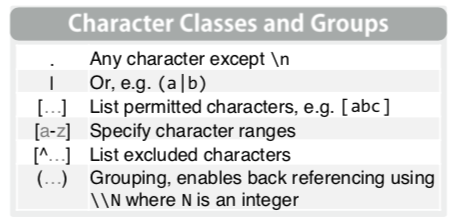
\includegraphics{/Users/lucas/Library/Mobile Documents/com~apple~CloudDocs/~~aa Study Materials/Grade 2 I/Learning/R for Data Science/Review of R/markdown/image/regexprs_classes_groups.png}
\item
  Special characters

  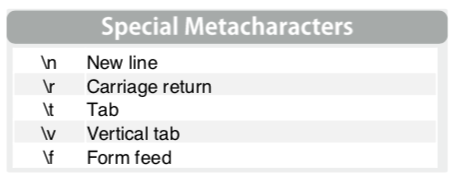
\includegraphics{/Users/lucas/Library/Mobile Documents/com~apple~CloudDocs/~~aa Study Materials/Grade 2 I/Learning/R for Data Science/Review of R/markdown/image/regexprs_special_characters.png}
\end{enumerate}

\begin{center}\rule{0.5\linewidth}{0.5pt}\end{center}

\hypertarget{r-for-bioinformatics-data-iteration--parallel-computing}{%
\section{R for bioinformatics, data iteration \& parallel
computing}\label{r-for-bioinformatics-data-iteration--parallel-computing}}

\begin{quote}
Talk 08
\end{quote}

\hypertarget{toc-4}{%
\subsection{TOC}\label{toc-4}}

\begin{itemize}
\item
  for loop
\item
  \texttt{apply} functions
\item
  The essence of \texttt{dplyr} is traversal.
\item
  \texttt{map} functions in \texttt{purrr} package
\item
  Iteration and Parallel Computing
\end{itemize}

\hypertarget{iteration-basics}{%
\subsection{\texorpdfstring{Iteration Basics
}{Iteration Basics }}\label{iteration-basics}}

\hypertarget{for-loop--getting-data-ready}{%
\subsubsection{\texorpdfstring{\texttt{for\ loop} , getting data
ready}{for loop , getting data ready}}\label{for-loop--getting-data-ready}}

Lookat this example:

\begin{Shaded}
\begin{Highlighting}[]
\NormalTok{df }\OtherTok{=}
	\FunctionTok{tibble}\NormalTok{( }
    \AttributeTok{a =} \FunctionTok{rnorm}\NormalTok{(}\DecValTok{100}\NormalTok{), }
    \AttributeTok{b =} \FunctionTok{rnorm}\NormalTok{(}\DecValTok{100}\NormalTok{), }
    \AttributeTok{c =} \FunctionTok{rnorm}\NormalTok{(}\DecValTok{100}\NormalTok{), }
    \AttributeTok{d =} \FunctionTok{rnorm}\NormalTok{(}\DecValTok{100}\NormalTok{)}
\NormalTok{  )}

\CommentTok{\# Calculate row means }
\NormalTok{res1 }\OtherTok{=}
	\FunctionTok{vector}\NormalTok{(}\StringTok{"double"}\NormalTok{, }\FunctionTok{nrow}\NormalTok{(df))}
\ControlFlowTok{for}\NormalTok{(row\_idx }\ControlFlowTok{in} \DecValTok{1}\SpecialCharTok{:}\FunctionTok{nrow}\NormalTok{(df))\{}
\NormalTok{  res1[row\_idx] }\OtherTok{=}
  	\FunctionTok{mean}\NormalTok{( }\FunctionTok{as.numeric}\NormalTok{(df[row\_idx, ]))}
\NormalTok{\}}

\NormalTok{res2 }\OtherTok{=} \FunctionTok{c}\NormalTok{()}
\ControlFlowTok{for}\NormalTok{(row\_idx }\ControlFlowTok{in} \DecValTok{1}\SpecialCharTok{:}\FunctionTok{nrow}\NormalTok{(df))\{}
\NormalTok{  res2[}\FunctionTok{length}\NormalTok{(res2) }\SpecialCharTok{+} \DecValTok{1}\NormalTok{] }\OtherTok{=}
  	\FunctionTok{mean}\NormalTok{(}\FunctionTok{as.numeric}\NormalTok{(df[row\_idx, ]))}
\NormalTok{\}}

\CommentTok{\# Similar to Python}

\CommentTok{\# Calculate column means }
\NormalTok{res2 }\OtherTok{=}
	\FunctionTok{vector}\NormalTok{(}\StringTok{"double"}\NormalTok{, }\FunctionTok{ncol}\NormalTok{(df))}
\ControlFlowTok{for}\NormalTok{(col\_idx }\ControlFlowTok{in} \DecValTok{1}\SpecialCharTok{:}\FunctionTok{ncol}\NormalTok{(df))\{}
\NormalTok{  res2[col\_idx] }\OtherTok{=}
  	\FunctionTok{mean}\NormalTok{(df[[col\_idx]])}
\NormalTok{\}}
\end{Highlighting}
\end{Shaded}

You can replace it with \texttt{for\ loop}:

\begin{Shaded}
\begin{Highlighting}[]
\FunctionTok{rowMeans}\NormalTok{(df)}
\FunctionTok{colMeans}\NormalTok{(df)}
\end{Highlighting}
\end{Shaded}

Here are some other functions:

\begin{Shaded}
\begin{Highlighting}[]
\FunctionTok{rowSums}\NormalTok{(df)}
\FunctionTok{colSums}\NormalTok{(df)}
\end{Highlighting}
\end{Shaded}

\hypertarget{apply-functions}{%
\subsubsection{\texorpdfstring{\texttt{apply}
functions}{apply functions}}\label{apply-functions}}

You can use \texttt{apply} with customizable function.

\begin{Shaded}
\begin{Highlighting}[]
\NormalTok{df }\SpecialCharTok{\%\textgreater{}\%} \FunctionTok{apply}\NormalTok{(}
\NormalTok{  ., }
  \DecValTok{2}\NormalTok{, }
  \ControlFlowTok{function}\NormalTok{(x) \{ }
    \FunctionTok{return}\NormalTok{(}
      \FunctionTok{c}\NormalTok{(}
        \AttributeTok{n =} \FunctionTok{length}\NormalTok{(x), }
        \AttributeTok{mean =} \FunctionTok{mean}\NormalTok{(x), }
        \AttributeTok{median =} \FunctionTok{median}\NormalTok{(x) }
\NormalTok{      )}
\NormalTok{    )}
\NormalTok{  \} }
\NormalTok{)}
\end{Highlighting}
\end{Shaded}

\hypertarget{something-about-tapply}{%
\subsubsection{\texorpdfstring{Something about
\texttt{tapply()}:}{Something about tapply():}}\label{something-about-tapply}}

The \texttt{tapply()} function in R is used to apply a function over
subsets of a vector, splitting it by a factor or list of factors. It
stands for "table apply" and is particularly useful for summarizing data
by groups or categories.

Here\textquotesingle s a breakdown of its usage:

\begin{Shaded}
\begin{Highlighting}[]
\FunctionTok{tapply}\NormalTok{(X, INDEX, FUN)}
\end{Highlighting}
\end{Shaded}

\begin{itemize}
\item
  \texttt{X}: The vector (or array) on which you want to apply the
  function.
\item
  \texttt{INDEX}: A factor or list of factors that define the groups.
  These factors determine how the vector \texttt{X} is split.
\item
  \texttt{FUN}: The function to be applied to each subset of \texttt{X}.
\end{itemize}

For example:

\begin{Shaded}
\begin{Highlighting}[]
\CommentTok{\# Creating a sample vector and a corresponding factor}
\NormalTok{values }\OtherTok{=} \FunctionTok{c}\NormalTok{(}\DecValTok{10}\NormalTok{, }\DecValTok{20}\NormalTok{, }\DecValTok{30}\NormalTok{, }\DecValTok{40}\NormalTok{, }\DecValTok{50}\NormalTok{)}
\NormalTok{categories }\OtherTok{=} \FunctionTok{factor}\NormalTok{(}\FunctionTok{c}\NormalTok{(}\StringTok{"A"}\NormalTok{, }\StringTok{"B"}\NormalTok{, }\StringTok{"A"}\NormalTok{, }\StringTok{"B"}\NormalTok{, }\StringTok{"A"}\NormalTok{))}

\CommentTok{\# Applying the mean function over subsets defined by the categories}
\FunctionTok{tapply}\NormalTok{(values, categories, mean)}
\end{Highlighting}
\end{Shaded}

In this example, \texttt{tapply()} calculates the mean of the
\texttt{values} vector for each category defined by the
\texttt{categories} factor. It splits the \texttt{values} vector into
subsets based on the categories and applies the \texttt{mean()} function
to each subset, returning the mean values for categories "A" and "B".

The result would be something like:

\begin{Shaded}
\begin{Highlighting}[]
\NormalTok{A    B }
\NormalTok{30   30}
\end{Highlighting}
\end{Shaded}

This indicates that the mean value for category "A" is 30, and the mean
value for category "B" is also 30 in this case.

\texttt{lapply()}, \texttt{sapply()}, and similar functions work on
elements of lists or vectors. In contrast, \texttt{tapply()} focuses on
splitting a vector by factors and applying a function to these subsets,
providing aggregated results for each subset determined by the factors.

\hypertarget{diffrences-between-apply-in-base-r-and-the-package-dplyr}{%
\subsubsection{\texorpdfstring{Diffrences between \texttt{apply} in base
R and the package
\texttt{dplyr}:}{Diffrences between apply in base R and the package dplyr:}}\label{diffrences-between-apply-in-base-r-and-the-package-dplyr}}

\begin{enumerate}
\def\labelenumi{\arabic{enumi}.}
\item
  \textbf{\texttt{apply} functions in base R:}

  \begin{itemize}
  \item
    The \texttt{apply} family of functions (\texttt{apply()},
    \texttt{lapply()}, \texttt{sapply()}, \texttt{vapply()}, etc.) in
    base R are used for applying a function over margins of arrays or
    data structures like matrices, arrays, and lists.
  \item
    \texttt{apply()} is used primarily for applying functions to the
    rows or columns of matrices or arrays, while \texttt{lapply()} and
    \texttt{sapply()} are more focused on lists.
  \item
    These functions are useful for repetitive operations across rows or
    columns without explicitly using loops.
  \end{itemize}

  Example:

\begin{Shaded}
\begin{Highlighting}[]
 \CommentTok{\# Creating a matrix}
\NormalTok{ mat }\OtherTok{=} \FunctionTok{matrix}\NormalTok{(}\DecValTok{1}\SpecialCharTok{:}\DecValTok{12}\NormalTok{, }\AttributeTok{nrow =} \DecValTok{3}\NormalTok{, }\AttributeTok{ncol =} \DecValTok{4}\NormalTok{)}

 \CommentTok{\# Applying sum function to rows (1) or columns (2) of the matrix}
 \FunctionTok{apply}\NormalTok{(mat, }\DecValTok{1}\NormalTok{, sum)  }\CommentTok{\# Sums of each row}
 \FunctionTok{apply}\NormalTok{(mat, }\DecValTok{2}\NormalTok{, sum)  }\CommentTok{\# Sums of each column}
\end{Highlighting}
\end{Shaded}
\item
  \textbf{\texttt{dplyr} package:}

  \begin{itemize}
  \item
    \texttt{dplyr} is a powerful package in R for data manipulation and
    transformation. It provides a set of functions (\texttt{filter()},
    \texttt{mutate()}, \texttt{select()}, \texttt{group\_by()},
    \texttt{summarize()}, etc.) that enable easy and intuitive data
    manipulation.
  \item
    It\textquotesingle s designed to work well with data frames and
    offers a more streamlined and readable syntax for performing common
    data manipulation tasks.
  \end{itemize}

  Example:

\begin{Shaded}
\begin{Highlighting}[]
 \FunctionTok{library}\NormalTok{(dplyr)}

 \CommentTok{\# Creating a sample data frame}
\NormalTok{ df }\OtherTok{=} \FunctionTok{data.frame}\NormalTok{(}
   \AttributeTok{Name =} \FunctionTok{c}\NormalTok{(}\StringTok{"Alice"}\NormalTok{, }\StringTok{"Bob"}\NormalTok{, }\StringTok{"Charlie"}\NormalTok{),}
   \AttributeTok{Age =} \FunctionTok{c}\NormalTok{(}\DecValTok{25}\NormalTok{, }\DecValTok{30}\NormalTok{, }\DecValTok{28}\NormalTok{),}
   \AttributeTok{Salary =} \FunctionTok{c}\NormalTok{(}\DecValTok{40000}\NormalTok{, }\DecValTok{50000}\NormalTok{, }\DecValTok{45000}\NormalTok{)}
\NormalTok{ )}

 \CommentTok{\# Filtering and selecting specific rows and columns}
\NormalTok{ filtered\_df }\OtherTok{=}\NormalTok{ df }\SpecialCharTok{\%\textgreater{}\%}
   \FunctionTok{filter}\NormalTok{(Age }\SpecialCharTok{\textgreater{}} \DecValTok{25}\NormalTok{) }\SpecialCharTok{\%\textgreater{}\%}
   \FunctionTok{select}\NormalTok{(Name, Salary)}

\NormalTok{ filtered\_df}
\end{Highlighting}
\end{Shaded}

  This \texttt{dplyr} example filters rows where \texttt{Age} is greater
  than 25 and selects only the \texttt{Name} and \texttt{Salary}
  columns. The \texttt{\%\textgreater{}\%} operator (pipe) chains
  together multiple operations, making the code more readable and
  concise.
\end{enumerate}

In summary, the \texttt{apply} family in base R is ideal for applying
functions to matrices, arrays, or lists across rows or columns, while
\texttt{dplyr} focuses on intuitive data manipulation operations for
data frames, providing a cleaner syntax and ease of use for common data
transformation tasks.

\hypertarget{more-on-iteration-purrr-package}{%
\subsection{\texorpdfstring{More on iteration: \texttt{purrr}
package}{More on iteration: purrr package}}\label{more-on-iteration-purrr-package}}

\hypertarget{about-purrr-from-official-website-httpspurrrtidyverseorg}{%
\subsubsection{\texorpdfstring{About \texttt{purrr} (from official
website
\url{https://purrr.tidyverse.org})}{About purrr (from official website https://purrr.tidyverse.org)}}\label{about-purrr-from-official-website-httpspurrrtidyverseorg}}

\texttt{purrr} enhances R's functional programming (FP) toolkit by
providing a complete and consistent set of tools for working with
functions and vectors. If you've never heard of FP before, the best
place to start is the family of \texttt{map()}functions which allow you
to replace many for loops with code that is both more succinct and
easier to read. The best place to learn about the \texttt{map()}
functions is the \href{https://r4ds.had.co.nz/iteration.html}{iteration
chapter} in R for data science.

\textbf{Usage}

The following example uses \texttt{purrr}to solve a fairly realistic
problem: split a data frame into pieces, fit a model to each piece,
compute the summary, then extract the R\textsuperscript{2}.

\begin{Shaded}
\begin{Highlighting}[]
\FunctionTok{library}\NormalTok{(purrr)}

\NormalTok{mtcars }\SpecialCharTok{|\textgreater{}} 
  \FunctionTok{split}\NormalTok{(mtcars}\SpecialCharTok{\$}\NormalTok{cyl) }\SpecialCharTok{|\textgreater{}}  \CommentTok{\# from base R}
  \FunctionTok{map}\NormalTok{(\textbackslash{}(df) }\FunctionTok{lm}\NormalTok{(mpg }\SpecialCharTok{\textasciitilde{}}\NormalTok{ wt, }\AttributeTok{data =}\NormalTok{ df)) }\SpecialCharTok{|\textgreater{}} 
  \FunctionTok{map}\NormalTok{(summary) }\SpecialCharTok{\%\textgreater{}\%}
  \FunctionTok{map\_dbl}\NormalTok{(}\StringTok{"r.squared"}\NormalTok{)}
  
\CommentTok{\#\textgreater{}         4         6         8 }
\CommentTok{\#\textgreater{} 0.5086326 0.4645102 0.4229655}
\end{Highlighting}
\end{Shaded}

This example illustrates some of the advantages of \texttt{purrr}
functions over the equivalents in base R:

\begin{itemize}
\item
  The first argument is always the data, so purrr works naturally with
  the pipe.
\item
  All \texttt{purrr} functions are type-stable. They always return the
  advertised output type (\texttt{map()} returns lists;
  \texttt{map\_dbl()} returns double vectors), or they throw an error.
\item
  All \texttt{map()} functions accept functions (named, anonymous, and
  lambda), character vector (used to extract components by name), or
  numeric vectors (used to extract by position).
\end{itemize}

\hypertarget{detailed-usage}{%
\subsubsection{Detailed Usage}\label{detailed-usage}}

\texttt{purrr} is a powerful package in R that focuses on enhancing and
simplifying the process of working with functions and vectors. Developed
as part of the tidyverse ecosystem, \texttt{purrr} provides a consistent
and coherent set of tools for functional programming, iteration, and
working with lists and vectors.

Here are some key aspects and functionalities of \texttt{purrr}:

\begin{enumerate}
\def\labelenumi{\arabic{enumi}.}
\item
  \textbf{Functional Programming:}

  \begin{itemize}
  \item
    \texttt{purrr} promotes functional programming paradigms in R,
    enabling users to work with functions as first-class objects.
  \item
    It provides functions like \texttt{map()}, \texttt{map2()},
    \texttt{pmap()}, \texttt{walk()}, and more, which allow applying
    functions over elements of lists or vectors.
  \end{itemize}
\item
  \textbf{Consistency Across Data Structures:}

  \begin{itemize}
  \item
    \texttt{purrr} functions exhibit consistent behavior across various
    data structures, such as lists, vectors, and data frames.
  \item
    These functions can work seamlessly with different data structures,
    making code more readable and maintainable.
  \end{itemize}
\item
  \textbf{Iteration and Mapping:}

  \begin{itemize}
  \item
    \texttt{map()} is a key function in \texttt{purrr} that iterates
    over elements of a list or vector, applying a function to each
    element and returning the results.
  \item
    \texttt{map2()} is similar to \texttt{map()} but allows iterating
    over two vectors simultaneously.
  \item
    \texttt{pmap()} extends this functionality to iterate over multiple
    vectors or lists simultaneously.
  \end{itemize}
\item
  \textbf{Simplified and Cleaner Syntax:}

  \begin{itemize}
  \item
    \texttt{purrr} functions often provide a more consistent and cleaner
    syntax compared to base R functions for similar operations.
  \item
    The use of the pipe \texttt{\%\textgreater{}\%} from the tidyverse
    allows chaining \texttt{purrr} functions together, resulting in more
    readable code.
  \end{itemize}
\item
  \textbf{Working with Lists and Data Frames:}

  \begin{itemize}
  \item
    \texttt{purrr} provides functions to efficiently manipulate and
    iterate over elements in lists and data frames.
  \item
    Functions like \texttt{map()} and \texttt{map\_dbl()} can be used to
    apply functions to each column of a data frame and collect results
    in an output structure.
  \end{itemize}
\end{enumerate}

Example of \texttt{map()} in \texttt{purrr}:

\begin{Shaded}
\begin{Highlighting}[]
\FunctionTok{library}\NormalTok{(purrr)}

\CommentTok{\# Applying sqrt function to each element of a list}
\NormalTok{numbers }\OtherTok{=} \FunctionTok{list}\NormalTok{(}\AttributeTok{a =} \DecValTok{1}\SpecialCharTok{:}\DecValTok{5}\NormalTok{, }\AttributeTok{b =} \DecValTok{6}\SpecialCharTok{:}\DecValTok{10}\NormalTok{)}
\NormalTok{result }\OtherTok{=} \FunctionTok{map}\NormalTok{(numbers, sqrt)}

\NormalTok{result}
\CommentTok{\# Output: List of 2}
\CommentTok{\# $ a: num [1:5] 1 1.41 1.73 2 2.24}
\CommentTok{\# $ b: num [1:5] 2.45 2.65 2.83 3 3.16}
\end{Highlighting}
\end{Shaded}

This code applies the \texttt{sqrt()} function to each element of the
list \texttt{numbers}, returning a list with the square roots of each
element.

\texttt{purrr} simplifies and enhances functional programming in R,
offering a consistent and expressive way to work with functions, lists,
vectors, and data frames, making data manipulation and iteration more
straightforward and concise.

\hypertarget{examples}{%
\subsubsection{Examples}\label{examples}}

Here are some specific functionalities and examples of \texttt{purrr}:

\begin{enumerate}
\def\labelenumi{\arabic{enumi}.}
\item
  \textbf{Mapping Functions:}

  \texttt{map()} applies a function to each element of a list or vector,
  returning a list.

\begin{Shaded}
\begin{Highlighting}[]
 \FunctionTok{library}\NormalTok{(purrr)}

 \CommentTok{\# Squaring each element in a vector using map()}
\NormalTok{ numbers }\OtherTok{=} \DecValTok{1}\SpecialCharTok{:}\DecValTok{5}
\NormalTok{ squared }\OtherTok{=} \FunctionTok{map}\NormalTok{(numbers, }\SpecialCharTok{\textasciitilde{}}\NormalTok{ .x}\SpecialCharTok{\^{}}\DecValTok{2}\NormalTok{)}

\NormalTok{ squared}
 \CommentTok{\# Output: List of 5}
 \CommentTok{\# \$ : int 1}
 \CommentTok{\# \$ : int 4}
 \CommentTok{\# \$ : int 9}
 \CommentTok{\# \$ : int 16}
 \CommentTok{\# \$ : int 25}
\end{Highlighting}
\end{Shaded}
\item
  \textbf{Mapping Functions over Multiple Inputs:}

  \texttt{map2()} allows applying a function that takes two inputs to
  corresponding elements of two vectors.

\begin{Shaded}
\begin{Highlighting}[]
 \CommentTok{\# Multiplying elements of two vectors element{-}wise}
\NormalTok{ vector1 }\OtherTok{=} \DecValTok{1}\SpecialCharTok{:}\DecValTok{5}
\NormalTok{ vector2 }\OtherTok{=} \DecValTok{6}\SpecialCharTok{:}\DecValTok{10}
\NormalTok{ product }\OtherTok{=} \FunctionTok{map2}\NormalTok{(vector1, vector2, }\SpecialCharTok{\textasciitilde{}}\NormalTok{ .x }\SpecialCharTok{*}\NormalTok{ .y)}

\NormalTok{ product}
 \CommentTok{\# Output: List of 5}
 \CommentTok{\# \$ : int 6}
 \CommentTok{\# \$ : int 14}
 \CommentTok{\# \$ : int 24}
 \CommentTok{\# \$ : int 36}
 \CommentTok{\# \$ : int 50}
\end{Highlighting}
\end{Shaded}
\item
  \textbf{Working with Data Frames:}

  \texttt{map\_df()} and similar functions allow applying a function to
  each column of a data frame and combining results into a data frame.

\begin{Shaded}
\begin{Highlighting}[]
 \CommentTok{\# Creating a data frame}
\NormalTok{ df }\OtherTok{=} \FunctionTok{data.frame}\NormalTok{(}\AttributeTok{A =} \DecValTok{1}\SpecialCharTok{:}\DecValTok{5}\NormalTok{, }\AttributeTok{B =} \DecValTok{6}\SpecialCharTok{:}\DecValTok{10}\NormalTok{)}

 \CommentTok{\# Doubling each column in the data frame}
\NormalTok{ doubled }\OtherTok{=} \FunctionTok{map\_df}\NormalTok{(df, }\SpecialCharTok{\textasciitilde{}}\NormalTok{ .x }\SpecialCharTok{*} \DecValTok{2}\NormalTok{)}

\NormalTok{ doubled}
 \CommentTok{\# Output: A tibble: 5 × 2}
 \CommentTok{\#       A     B}
 \CommentTok{\#   \textless{}dbl\textgreater{} \textless{}dbl\textgreater{}}
 \CommentTok{\# 1     2    12}
 \CommentTok{\# 2     4    14}
 \CommentTok{\# 3     6    16}
 \CommentTok{\# 4     8    18}
 \CommentTok{\# 5    10    20}
\end{Highlighting}
\end{Shaded}
\item
  \textbf{Iteration and Applying Functions:}

  \texttt{walk()} applies a function to each element without returning a
  result, useful for side effects or performing operations without
  output.

\begin{Shaded}
\begin{Highlighting}[]
\CommentTok{\# Printing each element of a list using walk()}
\NormalTok{fruits }\OtherTok{=} \FunctionTok{list}\NormalTok{(}\StringTok{"apple"}\NormalTok{, }\StringTok{"banana"}\NormalTok{, }\StringTok{"orange"}\NormalTok{)}
\FunctionTok{walk}\NormalTok{(fruits, print)}
\CommentTok{\# Output:}
\CommentTok{\# [1] "apple"}
\CommentTok{\# [1] "banana"}
\CommentTok{\# [1] "orange"}
\end{Highlighting}
\end{Shaded}
\end{enumerate}

\texttt{purrr} simplifies functional programming by providing intuitive
functions (\texttt{map()}, \texttt{map2()}, \texttt{walk()}, etc.) that
allow iteration over elements, applying functions, and collecting
results, making code more concise and readable in scenarios involving
lists, vectors, and data frames.

\hypertarget{in-the-slide-function-reduce-and-accumulate}{%
\subsubsection{\texorpdfstring{(in the slide) Function \texttt{reduce()}
and
\texttt{accumulate()}}{(in the slide) Function reduce() and accumulate()}}\label{in-the-slide-function-reduce-and-accumulate}}

Both \texttt{reduce()} and \texttt{accumulate()} are powerful functions
from the \texttt{purrr} package that facilitate iterative calculations
over a sequence, accumulating or reducing values based on a specified
function.

Here\textquotesingle s an explanation of each:

\begin{enumerate}
\def\labelenumi{\arabic{enumi}.}
\item
  \textbf{\texttt{reduce()} Function:}

  \begin{itemize}
  \item
    \texttt{reduce()} is used to successively apply a function to pairs
    of elements in a sequence, reducing it to a single value.
  \item
    The function provided to \texttt{reduce()} should take two arguments
    and return a single value.
  \item
    It starts by applying the function to the first two elements, then
    uses the result along with the next element, and so on, until the
    sequence is exhausted.
  \end{itemize}

  Example of \texttt{reduce()}:

\begin{Shaded}
\begin{Highlighting}[]
\FunctionTok{library}\NormalTok{(purrr)}

\CommentTok{\# Summing all elements in a vector using reduce()}
\NormalTok{numbers }\OtherTok{=} \DecValTok{1}\SpecialCharTok{:}\DecValTok{5}
\NormalTok{total\_sum }\OtherTok{=} \FunctionTok{reduce}\NormalTok{(numbers, }\StringTok{\textasciigrave{}}\AttributeTok{+}\StringTok{\textasciigrave{}}\NormalTok{)}

\NormalTok{total\_sum}
\CommentTok{\# Output: 15 (1 + 2 + 3 + 4 + 5 = 15)}
\end{Highlighting}
\end{Shaded}

  Here, \texttt{reduce()} adds all the elements in the \texttt{numbers}
  vector by applying the addition function (\texttt{+}) iteratively.
\item
  \textbf{\texttt{accumulate()} Function:}

  \begin{itemize}
  \item
    \texttt{accumulate()} is similar to \texttt{reduce()} but returns a
    sequence of intermediate results instead of a single value.
  \item
    It applies a function cumulatively to the sequence and returns a
    vector of values, representing the intermediate results at each
    step.
  \end{itemize}

  Example of \texttt{accumulate()}:

\begin{Shaded}
\begin{Highlighting}[]
\CommentTok{\# Calculating cumulative product of elements in a vector using accumulate()}
\NormalTok{factors }\OtherTok{=} \FunctionTok{c}\NormalTok{(}\DecValTok{2}\NormalTok{, }\DecValTok{3}\NormalTok{, }\DecValTok{4}\NormalTok{, }\DecValTok{5}\NormalTok{)}
\NormalTok{cumulative\_product }\OtherTok{=} \FunctionTok{accumulate}\NormalTok{(factors, }\StringTok{\textasciigrave{}}\AttributeTok{*}\StringTok{\textasciigrave{}}\NormalTok{)}

\NormalTok{cumulative\_product}
\CommentTok{\# Output: 2 6 24 120 (2, 2*3, 2*3*4, 2*3*4*5)}
\end{Highlighting}
\end{Shaded}

  Here, \texttt{accumulate()} applies the multiplication function
  (\texttt{*}) to each element in \texttt{factors}, returning a vector
  of cumulative products at each step.
\end{enumerate}

\texttt{reduce()} aggregates a sequence into a single value based on a
function, while \texttt{accumulate()} returns a sequence of intermediate
results. Both functions are helpful for iterative calculations and
provide different ways to process sequences of values in R.

\hypertarget{parallel-computing}{%
\subsection{Parallel Computing}\label{parallel-computing}}

\hypertarget{related-packages}{%
\subsubsection{Related Packages}\label{related-packages}}

\begin{itemize}
\item
  \texttt{parallel} package: displays the number of CPU cores to assign
  all or part to a task.
\item
  \texttt{foreach} package: provides \texttt{\%do\%} and
  \texttt{\%dopar\%} operators to submit tasks for sequential or
  parallel computation
\item
  \texttt{\textasciigrave{}\ iterators} package: splits
  \texttt{data.frame,\ tibble,\ matrix} into rows/columns for submitting
  parallel tasks.
\end{itemize}

\hypertarget{step-by-step-guidance}{%
\subsubsection{Step-by-step Guidance}\label{step-by-step-guidance}}

\begin{enumerate}
\def\labelenumi{\arabic{enumi}.}
\item
  \textbf{Prepare Data:}

  Assume you have a large data frame named \texttt{my\_data} that you
  want to process in parallel.
\item
  \textbf{Setup Parallel Processing:}

  Load necessary packages and initialize parallel processing
  capabilities.

\begin{Shaded}
\begin{Highlighting}[]
 \FunctionTok{library}\NormalTok{(parallel)}
 \FunctionTok{library}\NormalTok{(doParallel)}
 \FunctionTok{library}\NormalTok{(foreach)}
 \FunctionTok{library}\NormalTok{(iterators)}

 \CommentTok{\# Set the number of cores/processors to be used}
\NormalTok{ num\_cores }\OtherTok{=} \FunctionTok{detectCores}\NormalTok{()}

 \CommentTok{\# Initialize parallel backend}
\NormalTok{ cl }\OtherTok{=} \FunctionTok{makeCluster}\NormalTok{(num\_cores)}
 \FunctionTok{registerDoParallel}\NormalTok{(cl)}
\end{Highlighting}
\end{Shaded}
\item
  \textbf{Split Data Frame into Chunks:}

  Use the \texttt{iter()} function from the \texttt{iterators} package
  to create an iterator for chunks of your data frame.

\begin{Shaded}
\begin{Highlighting}[]
 \CommentTok{\# Define chunk size}
\NormalTok{ chunk\_size }\OtherTok{=} \FunctionTok{nrow}\NormalTok{(my\_data) }\SpecialCharTok{/}\NormalTok{ num\_cores}

 \CommentTok{\# Create an iterator for the chunks}
\NormalTok{ my\_iterator }\OtherTok{=} \FunctionTok{iter}\NormalTok{(my\_data, }\AttributeTok{by =} \StringTok{"row"}\NormalTok{, }\AttributeTok{chunksize =}\NormalTok{ chunk\_size)}
\end{Highlighting}
\end{Shaded}
\item
  \textbf{Perform Parallel Computation:}

  Use \texttt{foreach()} from the \texttt{foreach} package along with
  \texttt{\%dopar\%} to apply a function to each chunk in parallel.

\begin{Shaded}
\begin{Highlighting}[]
 \CommentTok{\# Define a function to process each chunk}
\NormalTok{ process\_chunk }\OtherTok{=} \ControlFlowTok{function}\NormalTok{(chunk) \{}
   \CommentTok{\# Your processing logic for each chunk goes here}
   \CommentTok{\# For example: summary(chunk)}
   \CommentTok{\# Replace summary() with your specific data processing task}
\NormalTok{ \}}

 \CommentTok{\# Apply the function to each chunk in parallel}
\NormalTok{ results }\OtherTok{=} \FunctionTok{foreach}\NormalTok{(}\AttributeTok{chunk =}\NormalTok{ my\_iterator, }\AttributeTok{.combine =}\NormalTok{ rbind) }\SpecialCharTok{\%dopar\%}\NormalTok{ \{}
   \FunctionTok{process\_chunk}\NormalTok{(chunk)}
\NormalTok{ \}}
\end{Highlighting}
\end{Shaded}
\item
  \textbf{Combine Results:}

  Collect and combine the results obtained from parallel processing.

\begin{Shaded}
\begin{Highlighting}[]
 \CommentTok{\# Combine or process the results obtained from parallel computation}
\NormalTok{ final\_result }\OtherTok{=} \FunctionTok{do.call}\NormalTok{(rbind, results)}

 \CommentTok{\# Close the parallel cluster}
 \FunctionTok{stopCluster}\NormalTok{(cl)}
\end{Highlighting}
\end{Shaded}
\end{enumerate}

Replace the \texttt{process\_chunk()} function with your specific data
processing task. This approach parallelizes the processing of chunks of
the data frame across multiple cores, allowing for faster computations,
especially with large datasets.

\textbf{Note:}

\begin{itemize}
\item
  When the task is completed, the allocated CPU core is reclaimed.
\item
  Ensure that your specific data processing task is compatible with
  parallelization and that the benefits of parallel computing outweigh
  the overhead of parallelization.
\item
  Also, consider potential dependencies or shared resources among
  iterations when parallelizing computations.
\end{itemize}

\hypertarget{in-the-slide-function-foreach}{%
\subsubsection{\texorpdfstring{(in the slide) Function
\texttt{foreach()}}{(in the slide) Function foreach()}}\label{in-the-slide-function-foreach}}

\hypertarget{simple-usage}{%
\paragraph{\texorpdfstring{\textbf{Simple usage}}{Simple usage}}\label{simple-usage}}

\hypertarget{description-3}{%
\paragraph{Description}\label{description-3}}

\texttt{⁠\%do\%⁠} and \texttt{⁠\%dopar\%⁠} are binary operators that operate
on a \texttt{foreach} object and an \texttt{R} expression. The
expression, \texttt{ex}, is evaluated multiple times in an environment
that is created by the \texttt{foreach} object, and that environment is
modified for each evaluation as specified by the \texttt{foreach}
object. \texttt{⁠\%do\%⁠} evaluates the expression sequentially, while
\texttt{⁠\%dopar\%⁠} evaluates it in parallel. The results of evaluating
\texttt{ex} are returned as a list by default, but this can be modified
by means of the \texttt{.combine} argument.

\hypertarget{usage-2}{%
\paragraph{Usage}\label{usage-2}}

\begin{Shaded}
\begin{Highlighting}[]
\FunctionTok{foreach}\NormalTok{(}
\NormalTok{  ...,}
\NormalTok{  .combine,}
\NormalTok{  .init,}
  \AttributeTok{.final =} \ConstantTok{NULL}\NormalTok{,}
  \AttributeTok{.inorder =} \ConstantTok{TRUE}\NormalTok{,}
  \AttributeTok{.multicombine =} \ConstantTok{FALSE}\NormalTok{,}
  \AttributeTok{.maxcombine =} \ControlFlowTok{if}\NormalTok{ (.multicombine) }\DecValTok{100} \ControlFlowTok{else} \DecValTok{2}\NormalTok{,}
  \AttributeTok{.errorhandling =} \FunctionTok{c}\NormalTok{(}\StringTok{"stop"}\NormalTok{, }\StringTok{"remove"}\NormalTok{, }\StringTok{"pass"}\NormalTok{),}
  \AttributeTok{.packages =} \ConstantTok{NULL}\NormalTok{,}
  \AttributeTok{.export =} \ConstantTok{NULL}\NormalTok{,}
  \AttributeTok{.noexport =} \ConstantTok{NULL}\NormalTok{,}
  \AttributeTok{.verbose =} \ConstantTok{FALSE}
\NormalTok{)}
\NormalTok{e1 }\SpecialCharTok{\%:\%}\NormalTok{ e2}
\FunctionTok{when}\NormalTok{(cond)}
\NormalTok{obj }\SpecialCharTok{\%do\%}\NormalTok{ ex}
\NormalTok{obj }\SpecialCharTok{\%dopar\%}\NormalTok{ ex}
\FunctionTok{times}\NormalTok{(n)}
\end{Highlighting}
\end{Shaded}

\hypertarget{nested-foreach}{%
\subsubsection{\texorpdfstring{Nested
\texttt{foreach}}{Nested foreach}}\label{nested-foreach}}

\begin{quote}
Expanded knowledge, not featured on slide, for understanding only.
\end{quote}

Nested \texttt{foreach} loops in R allow for the iteration over multiple
levels of nested structures or combinations of iterators. This approach
is particularly useful when dealing with hierarchical data or when you
need to perform computations on multiple levels of nested objects
simultaneously.

Here\textquotesingle s an overview of nested \texttt{foreach} loops:

\begin{enumerate}
\def\labelenumi{\arabic{enumi}.}
\item
  \textbf{Nested Iteration:}

  \texttt{foreach} supports nesting, allowing you to iterate over
  multiple levels of nested structures, such as lists within lists or
  matrices within lists.

\begin{Shaded}
\begin{Highlighting}[]
\FunctionTok{library}\NormalTok{(foreach)}

\CommentTok{\# Example: Nested foreach loop iterating over a list of lists}
\NormalTok{outer\_list }\OtherTok{=} \FunctionTok{list}\NormalTok{(}\FunctionTok{list}\NormalTok{(}\AttributeTok{a =} \DecValTok{1}\NormalTok{, }\AttributeTok{b =} \DecValTok{2}\NormalTok{), }\FunctionTok{list}\NormalTok{(}\AttributeTok{c =} \DecValTok{3}\NormalTok{, }\AttributeTok{d =} \DecValTok{4}\NormalTok{))}

\FunctionTok{foreach}\NormalTok{(}\AttributeTok{inner\_list =}\NormalTok{ outer\_list) }\SpecialCharTok{\%:\%}\NormalTok{ \{}
  \FunctionTok{foreach}\NormalTok{(}\AttributeTok{element =}\NormalTok{ inner\_list) }\SpecialCharTok{\%do\%}\NormalTok{ \{}
    \CommentTok{\# Process each element within the nested structure}
    \FunctionTok{print}\NormalTok{(element)}
\NormalTok{  \}}
\NormalTok{\}}
\end{Highlighting}
\end{Shaded}

  This code iterates over each element of \texttt{outer\_list}, which
  contains inner lists. Within each inner list, it iterates over the
  elements.
\item
  \textbf{Combining Iterators:}

  You can combine different iterators using \texttt{\%:\%} to create
  nested iterations.

\begin{Shaded}
\begin{Highlighting}[]
\CommentTok{\# Example: Nested foreach loop with combined iterators}
\NormalTok{values }\OtherTok{=} \DecValTok{1}\SpecialCharTok{:}\DecValTok{3}
\NormalTok{letters }\OtherTok{=}\NormalTok{ letters[}\DecValTok{1}\SpecialCharTok{:}\DecValTok{4}\NormalTok{]}

\FunctionTok{foreach}\NormalTok{(}\AttributeTok{i =}\NormalTok{ values) }\SpecialCharTok{\%:\%} \FunctionTok{foreach}\NormalTok{(}\AttributeTok{letter =}\NormalTok{ letters) }\SpecialCharTok{\%do\%}\NormalTok{ \{}
  \CommentTok{\# Perform operations using both iterators}
  \FunctionTok{print}\NormalTok{(}\FunctionTok{paste}\NormalTok{(}\StringTok{"Value:"}\NormalTok{, i, }\StringTok{"| Letter:"}\NormalTok{, letter))}
\NormalTok{\}}
\end{Highlighting}
\end{Shaded}

  This code creates nested iterations, iterating over \texttt{values}
  and \texttt{letters} simultaneously.
\item
  \textbf{Applying Nested Functions:}

  Nested \texttt{foreach} loops are valuable when applying functions or
  performing operations that require iterating over multiple levels of
  nested data structures or combinations.

\begin{Shaded}
\begin{Highlighting}[]
\CommentTok{\# Example: Applying a function with nested foreach loops}
\NormalTok{matrix\_list }\OtherTok{=} \FunctionTok{list}\NormalTok{(}\FunctionTok{matrix}\NormalTok{(}\DecValTok{1}\SpecialCharTok{:}\DecValTok{4}\NormalTok{, }\AttributeTok{nrow =} \DecValTok{2}\NormalTok{), }\FunctionTok{matrix}\NormalTok{(}\DecValTok{5}\SpecialCharTok{:}\DecValTok{8}\NormalTok{, }\AttributeTok{nrow =} \DecValTok{2}\NormalTok{))}

\FunctionTok{foreach}\NormalTok{(}\AttributeTok{mat =}\NormalTok{ matrix\_list) }\SpecialCharTok{\%:\%} \FunctionTok{foreach}\NormalTok{(}\AttributeTok{element =} \FunctionTok{as.vector}\NormalTok{(mat)) }\SpecialCharTok{\%do\%}\NormalTok{ \{}
  \CommentTok{\# Perform computations on each element of each matrix}
  \FunctionTok{print}\NormalTok{(element }\SpecialCharTok{*} \DecValTok{2}\NormalTok{)}
\NormalTok{\}}
\end{Highlighting}
\end{Shaded}

  Here, it iterates over a list of matrices and then iterates over each
  element within the matrices to perform computations.
\end{enumerate}

Nested \texttt{foreach} loops in R allow for flexible and efficient
iterations over hierarchical or nested structures, enabling complex
computations, data manipulations, or simulations involving multiple
levels of nested objects or iterators.

\end{document}
